\documentclass[twoside,10pt,a4paper]{article}
\usepackage[utf8]{inputenc}
\usepackage[english]{babel}
\usepackage{amsmath}
\usepackage{amsfonts}
\usepackage{amssymb}
\usepackage{graphicx}

\usepackage[left=2cm,right=2cm,top=2cm,bottom=3cm]{geometry}
\usepackage{fancyvrb} 
\usepackage{listings}
\usepackage{xparse}
\usepackage{tikz} % ajout de dessins LaTeX
\usepackage{graphicx}
\usepackage{float}  % alignement des figures
\usepackage{fancyhdr}
\usepackage{enumitem}
\usepackage{verbatim}
\usepackage{xcolor}
\usepackage{bm}

\usepackage{caption}
\usepackage{subcaption}

\pagestyle{fancy} %fancyhdr
	\fancyhf{} %fancyhdr
	\renewcommand{\sectionmark}[1]{\markboth{#1}{}}
	\fancyhead[R]{NLDCI Set 2 Solutions} %INSERT TITLE HERE FOR fancyhdr
	\fancyhead[L]{\nouppercase{\leftmark}} %fancyhdr
	\cfoot{\thepage} %fancyhdr
	\setlength{\headheight}{35pt}
	\setlength{\parindent}{0pt}

\begin{titlepage}
\title{\huge \textbf{Nonlinear Dynamics \& Chaos I \\ \Large Exercice Set 2 Solutions}}	%TITLE
\author{ }		%AUTHOR
\date{ }	%DATE

\end{titlepage}


\begin{document}

\maketitle

\section*{Question 1}
Consider the nonlinear oscillator
\begin{equation*}
	\ddot{x} + \omega_0^2 x= \varepsilon Mx^2,
\end{equation*}
where $\varepsilon M x^2$ represents a small nonlinear forcing term $(0 \leq \varepsilon \ll 1, M > 0)$.

Using Lindstedt's method, find an $\mathcal{O}(\varepsilon)$ approximation for nonlinear motions as a function of their initial position, with zero initial velocity.

\section*{Solution 1}
\begin{align*}
	\ddot{x} + \omega_0^2 x &= \varepsilon Mx^2, \quad 0 < \varepsilon \ll 1, \quad M>0, \quad \omega_0 \neq 0 \\
	x(0) &= a_0 \\
	\dot{x}(0) &= 0
\end{align*}
\begin{itemize}
	\item Seek solutions of the form:
		\begin{align*}
			x_\varepsilon(t) &= \varphi_0(t;\varepsilon) + \varepsilon\varphi_1(t;\varepsilon) + \mathcal{O}(\varepsilon^2) \\
			\varphi_i (t, \varepsilon) &= \varphi_i(t + T_\varepsilon; \varepsilon)
		\end{align*}
	\item rewrite period as
		\begin{equation*}
			T_\varepsilon = \frac{2\pi}{\omega(\varepsilon)}, \quad \omega(\varepsilon) = \omega_0 + \varepsilon \omega_1 + \mathcal{O}(\varepsilon^2)
		\end{equation*}
	\item Rescale time: 
		\begin{equation}
			\tau = \omega(\varepsilon)t \Longrightarrow \boxed{\frac{d}{d\tau} = \frac{1}{\omega(\varepsilon)}\frac{d}{dt}} \Longrightarrow \boxed{\left(\omega(\varepsilon)\right)^2x''+\omega_0^2 x = \varepsilon M x^2}
		\end{equation}
	\item Plug in the new Ansatz into the rescaled equation
		\begin{equation*}
			[\omega_0^2 + 2\varepsilon \omega_0 \omega_1 + \mathcal{O}(\varepsilon^2)][\varphi_0'' + \varepsilon \varphi_1''+ \mathcal{O}(\varepsilon^2)] + \omega_0^2[\varphi_0 + \varepsilon \varphi_1+ \mathcal{O}(\varepsilon^2)] = \varepsilon M [\varphi_0^2 + \mathcal{O}(\varepsilon)]
		\end{equation*}
	\item Collect terms of equal power of $\varepsilon$
	
	$\mathcal{O}(1)$:
	\begin{align*}
		\omega_0^2\varphi_0'' + \omega_0^2 \varphi_0 &= 0, \quad \varphi_0(0) = a_0, \quad \dot{\varphi}_0(0)=0 \\
		\Longrightarrow \varphi_0 &= a_0 \cos(\tau)
	\end{align*}
	$\mathcal{O}(2)$:
	\begin{align*}
		\omega_0^2\varphi_1'' + \omega_0^2 \varphi_1 &= M \varphi_0^2 - 2\omega_0\omega_1\varphi_0'' = Ma_0^2 \cos^2(\tau) + 2a_0\omega_0\omega_1 \cos(\tau) \\
		&= M \frac{a_0^2}{2}[1 + \cos(2\tau)] + \underbrace{2a_0\omega_0\omega_1\cos(\tau)}_{\text{resonance}}
	\end{align*}
	Select $\omega_1 = 0$ to eliminate resonance terms and obtain periodic solution.
	
	Solve for $\varphi_1$:
	\begin{equation} \label{S02E011}
		\varphi_1'' + \varphi_1 = \frac{Ma_0^2}{2\omega_0^2}[1 + \cos(2\tau)], \quad \varphi_1(0)=0, \quad \dot{\varphi}_1(0)=0
	\end{equation}
	\item Pick solution Ansatz:
	\begin{equation*}
		\varphi_1(\tau) = A\cos(\tau) + B\sin(\tau) + C\cos(2\tau) + D\sin(2\tau) + E
	\end{equation*}
	\item Substituting in (\ref{S02E011}):
	\begin{align*}
		-A\cos(\tau) - B\sin(\tau) - 4C\cos(2\tau) - 4D\sin(2\tau) + A\cos(\tau) + B\sin(\tau) + C\cos(2\tau) + D\sin(2\tau) + E \\
		= \frac{Ma_0^2}{2\omega_0^2}\cos(2\tau) + \frac{Ma_0^2}{2\omega_0^2}
	\end{align*}
	\item Comparing coefficients:
	\begin{equation*}
		\Longrightarrow E = \frac{Ma_0^2}{2\omega_0^2}, \quad C = -\frac{Ma_0^2}{6\omega_0^2},\quad D=0
	\end{equation*}
	\begin{align*}
		\varphi_1(0)=0 &\Longrightarrow A+C+E=0 \Longrightarrow A = -\frac{Ma_0^2}{3\omega_0^2} \\
		\varphi_1'(0)=0 &\Longrightarrow B+2D=0 \Longrightarrow B=0
	\end{align*}
	\begin{equation*}
		\Longrightarrow \boxed{\varphi_1(\tau) = -\frac{Ma_0^2}{3\omega_0^2}\cos(\tau) - \frac{Ma_0^2}{6\omega_0^2}\cos(2\tau) + \frac{Ma_0^2}{2\omega_0^2}}
	\end{equation*}
	\item In original time:
	\begin{equation*}
		x_\varepsilon(t) = a_0\cos(\omega t) + \varepsilon \frac{Ma_0^2}{\omega_0^2} \left[ -\frac{1}{3}\cos(\omega t) - \frac{1}{6}\cos(2\omega t) + \frac{1}{2} \right] + \mathcal{O}(\varepsilon^2)
	\end{equation*}
	where
	\begin{equation*}
		\omega = \omega_0 + \mathcal{O}(\varepsilon^2)
	\end{equation*}
\end{itemize}

\newpage
\section*{Question 2}
Consider the forced \textit{van der Pol equation}
\begin{equation*}
	\ddot{x} + \varepsilon(x^2 - 1)\dot{x} + x = F\cos(\omega t),
\end{equation*} 
which arises in models of self-excited oscillation, such as those of a valve generator with a cubic valve characteristic. Here $F, \omega > 0$ are parameters, and $0 \leq \varepsilon \ll 1$.

\begin{enumerate}[label=(\roman*)]
	\item For small values of $\varepsilon$, find an approximation for an \textbf{exactly} $2\pi/\omega$-periodic solution of the equation. The error of your approximation should be $\mathcal{O}(\varepsilon)$.
	\item For $\varepsilon = 0.1, \; \omega = 2$, and $F = 1$, verify your prediction numerically by solving the equation numerically. Plot your numerical solution along with your analytic prediction computed in (i).

\textit{Note}: For chaotic dynamics in the forced van der Pol equation, see Section 2.1 of \textit{Guckenheimer \& Holmes}.
\end{enumerate}

\section*{Solution 2}
\begin{enumerate}[label=(\roman*)]
\item Seek solutions of the form:
\begin{equation*}
	x_\varepsilon(t)=\varphi_0(t)+ \varepsilon\varphi_1(t) + \mathcal{O}(\varepsilon^2)
\end{equation*}
Substituting this solution in the ODE $\ddot{x} + \varepsilon(x^2-1)\dot{x} + x = F\cos(\omega t)$ we get:
\begin{equation*}
	\ddot{\varphi}_0 + \varphi_0 + \varepsilon(\ddot{\varphi}_1 + \varphi_1 + \varphi_0^2\dot{\varphi}_0 - \dot{\varphi}_0) + \mathcal{O}(\varepsilon^2) = F\cos(\omega t)
\end{equation*}
\begin{align}
	\Longrightarrow \mathcal{O}(1) &: \ddot{\varphi}_0 + \varphi_0 = F\cos(\omega t) \label{S02E021} \\
	\Longrightarrow \mathcal{O}(2) &: \ddot{\varphi}_1 + \varphi_1 = \dot{\varphi}_0(1-\varphi_0^2) \label{S02E022}
\end{align}
From equation (\ref{S02E021}):
\begin{equation}
	\varphi_0(t) = A\sin(t) + B\cos(t) + \frac{F\cos(\omega t)}{1-\omega^2} \label{S02E023}
\end{equation}
Since we seek solutions with period $\frac{2\pi}{\omega}$ for any $0\leq \varepsilon \ll 1$, the period of each $\varphi_i$ must be $\frac{2\pi}{\omega}$. This holds in particular for $\varphi_0$. Therefore, we must enforce $A=B=0$ in equation (\ref{S02E023}).

This condition can be enforced by choosing appropriate initial conditions for the ODE (\ref{S02E021}):
\begin{equation}\label{S02E024}
	A=B=0 \Longrightarrow \boxed{\varphi_0(t) = \frac{F\cos(\omega t)}{1-\omega^2}, \quad \varphi_0(0) = \frac{F}{1-\omega^2}, \quad \dot{\varphi}_0(0)=0}
\end{equation}
\begin{equation*}
	x_\varepsilon(t) = \varphi_0(t) + \underbrace{\mathcal{O}(\varepsilon)}_\text{error term}
\end{equation*}


\item We solve the ODE numerically to obtain a solution $x(t)$ and compare this solution to the perturbed approximation $x_\varepsilon(t)$ given by (\ref{S02E024}).

The initial conditions for the ODE are chosen such that $x(0) = x_\varepsilon(0)$ and $\dot{x}(0) = \dot{x}_\varepsilon(0)$.

Therefore, $x(0)=\varphi_0(0), \quad \dot{x}(0) = \dot{\varphi}_0(0)$ where $\varphi_0(0)$ and $\dot{\varphi}_0(0)$ are given in (\ref{S02E024}).

Equivalent first order system of differential equations:
\begin{equation}
	z_1 = x, \quad z_2 = \dot{x}, \quad \begin{bmatrix}
		\dot{z}_1 \\
		\dot{z}_2
	\end{bmatrix} = \begin{bmatrix}
		z_2 \\
		F\cos(\omega t) + \varepsilon(z_1^2 - 1)z_2 - z_1
	\end{bmatrix}
\end{equation}
\begin{figure}[H]
	\centering
	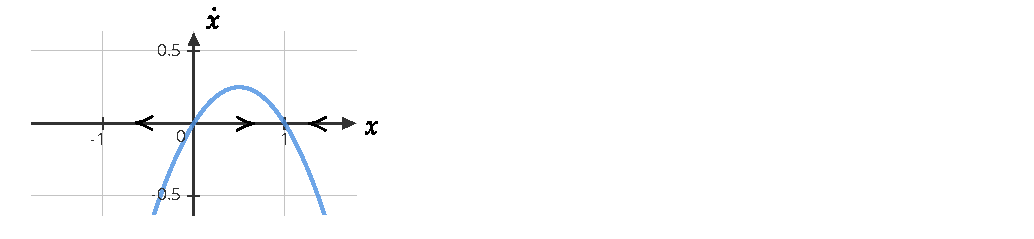
\includegraphics[scale=0.5]{Graphics/Q02D01.eps}
\end{figure}
\end{enumerate}

\subsection*{MATLAB code}
\begin{Verbatim}[numbers = left]
%% Initiate Script

close all
clear all
clc

%% define parameters

epsilon = 0.1;
omega = 2;
F = 1;

% initial condition
t0 = [F / (1 - omega.^2), 0]';

% time steps
tt_approx = 0:0.01:pi;
tt_sim = 0:0.01: 101 * pi;

%% Function and simulation

fun = @(t,x) [x(2); F*cos(omega * t) + epsilon * (x(1).^2 - 1).*x(2) - x(1)];

opts = odeset('RelTol',1e-4,'AbsTol',1e-6);
[~ , xtrue] = ode45(fun, tt_sim, t0, opts);

%% Approximation

xApprox = F * cos(omega .* tt_approx) / (1 - omega.^2);

%% Plot results

xtrue_steady_state = xtrue(end - length(xApprox) + 1: end, 1); % only take the last 315 values

figure(1)
hold on
plot(tt_approx, xtrue_steady_state,'linewidth',1.5,'DisplayName','ODE45');
plot(tt_approx, xApprox,'linewidth',1.5,'DisplayName','Approximation');
xlabel('$t$','interpreter','Latex','FontSize',16)
ylabel('$x$','interpreter','Latex','FontSize',16)
legnd1 = legend;
legnd1.NumColumns = 1;
legnd1.FontSize = 14;
hold off
grid on
\end{Verbatim}





\end{document}